\documentclass[11pt,letterpaper]{article}
\usepackage[lmargin=1in,rmargin=1in,bmargin=1in,tmargin=1in]{geometry}
\usepackage{style}

\setlength{\parindent}{0ex}

\usepackage{polynom}

% -------------------
% Content
% -------------------
\begin{document}

% Title
\begin{center} {\bfseries \LARGE MATH 142 --- Learning Outcomes --- Fall 2025} \end{center}

Here are some of the learning outcomes for each lecture. That is, after lecture, the homework, and studying, what students should know from each lecture. Though this list is not necessarily \textit{completely} comprehensive, the most important ideas/concepts are contained in each list. Students should be sure to feel comfortable with each bullet point before an exam. These learning goals are broken down by class date---with the class topic given. The classes are given in reverse-chronological order for ease of access to the most recent class. You may also click any of the hyperlinks below to jump to that date. 

\begin{itemize}
\item \hyperref[09-09]{09/09, Thursday: Partial Fractions}
\item \hyperref[09-04]{09/04, Thursday: Partial Fractions}
\item \hyperref[09-02]{09/02, Tuesday: Trig. Substitution}
\item \hyperref[08-28]{08/28, Thursday: Trigonometric Integrals}
\item \hyperref[08-26]{08/26, Tuesday: Integration-by-Parts}
\item \hyperref[08-21]{08/21, Thursday: Integration-by-Parts}
\item \hyperref[08-19]{08/19, Tuesday: $u$-Substitution Review}
\end{itemize}

% 09/09, Thursday: Partial Fractions
\newpage
\section*{09/09, Thursday: Partial Fractions\label{09-09}}

\begin{itemize}
\item Know what Heaviside's Method/Cover-Up Method (without modification) can find in a partial fraction decomposition (the term for the highest power of a linear term). For example, 
	\[
	\begin{aligned}
	\dfrac{\;\;\;\rule{1cm}{0.3pt}\;\;\;}{(x - 2)(x + 3)}&= \dfrac{\boxed{A}}{x - 2} + \dfrac{\boxed{B}}{x + 3} \\
	\dfrac{\;\;\;\rule{1cm}{0.3pt}\;\;\;}{x^2(x + 5)}&= \dfrac{A}{x} + \dfrac{\boxed{B}}{x^2} + \dfrac{\boxed{C}}{x + 5} \\
	\dfrac{\;\;\;\rule{1cm}{0.3pt}\;\;\;}{x(x^2 + 4)}&= \dfrac{\boxed{A}}{x} + \dfrac{Bx + C}{x^2 + 4} \\
	\dfrac{\;\;\;\rule{1cm}{0.3pt}\;\;\;}{x(x + 2)^2}&= \dfrac{\boxed{A}}{x} + \dfrac{B}{x + 2} + \dfrac{\boxed{C}}{(x + 2)^2}
	\end{aligned}
	\]
Heaviside's method (without modification) will only find the boxed coefficients above. Other work will be required to find the other terms. 

\item Be able to use Heaviside's method in a partial fractions integral, e.g. 
	\[
	\int \dfrac{x + 3}{(x - 1)(x + 2)} \;dx
	\]
	\[
	\dfrac{x + 3}{(x - 1)(x + 2)}= \dfrac{A}{x - 1} + \dfrac{B}{x + 2}
	\]
	\[
	A= \dfrac{1 + 3}{1 + 2}= \dfrac{4}{3} \qquad B= \dfrac{-2 + 3}{-2 - 1}= \dfrac{1}{-3}
	\]
	\[
	\int \dfrac{x + 3}{(x - 1)(x + 2)} \;dx= \int \dfrac{4/3}{x - 1} + \dfrac{-1/3}{x + 2} \;dx= \tfrac{4}{3} \ln|x - 1| - \tfrac{1}{3} \ln|x + 2| + K
	\]

\item Be able to complete a partial fractions integral when Heaviside's method fails to compute all terms. 

\item Know other `shortcut' methods for partial fractions, e.g. evaluating the expressions at various $x$-values. 
\end{itemize}

% 09/04, Thursday: Partial Fractions
\newpage
\section*{09/04, Thursday: Partial Fractions\label{09-04}}

\begin{itemize}
\item Be able to long divide polynomials, e.g.
	\[
	\polylongdiv{X^3+X^2-1}{X-1}
	\]

\item Recall that for a partial fraction decomposition, the degree of the numerator must be \textit{less than} the degree of the denominator.

\item Be able to write the `form' of a partial fraction decomposition, e.g.
	\[
	\begin{aligned}
	\dfrac{\;\;\;\rule{1cm}{0.3pt}\;\;\;}{(x - 2)(x + 3)}&= \dfrac{A}{x - 2} + \dfrac{B}{x + 3} \\
	\dfrac{\;\;\;\rule{1cm}{0.3pt}\;\;\;}{x^2(x + 5)}&= \dfrac{A}{x} + \dfrac{B}{x^2} + \dfrac{C}{x + 5} \\
	\dfrac{\;\;\;\rule{1cm}{0.3pt}\;\;\;}{x(x^2 + 4)}&= \dfrac{A}{x} + \dfrac{Bx + C}{x^2 + 4} \\
	\dfrac{\;\;\;\rule{1cm}{0.3pt}\;\;\;}{x(x + 2)^2}&= \dfrac{A}{x} + \dfrac{B}{x + 2} + \dfrac{C}{(x + 2)^2}
	\end{aligned}
	\]

\item Be able to identify when integrals may be a partial fractions integral---integrals of rational functions, e.g. $\ds\int \dfrac{x + 3}{(x - 1)(x + 5)} \;dx$, $\ds\int \dfrac{2x^3 - x^2 + 3x + 1}{x^2 + 1} \;dx$, $\ds\int \dfrac{5x + 3}{x^2 + 3x} \;dx$, $\ds\int \dfrac{x + 3}{x(x^2 - 1)} \;dx$, etc. 

\item Be able to compute integrals using partial fractions. 

\item Be able to integrate integrals of the form $\ds\int \dfrac{Ax}{x^2 + B} \;dx$ (using $u$-substitution, this is $\tfrac{A}{2} \ln|x^2 + B| + C$, e.g. $\ds\int \dfrac{3x}{x^2 + 9} \;dx$.

\item Be able to integrate integrals of the form $\ds\int \dfrac{B}{x^2 + A} \;dx$ (after algebra and a $u$-substitution, this is $\tfrac{B}{\sqrt{A}} \arctan\left( \tfrac{x}{\sqrt{A}} \right) + C$.
\end{itemize}

% 09/02, Tuesday: Trig. Substitution
\newpage
\section*{09/02, Tuesday: Trig. Substitution\label{09-02}}

\begin{itemize}
\item Be able to recognize integrals which may require trig. substitution---integrals containing terms `coming from the Pythagorean Theorem', e.g. $x^2 + 4$, $9 - x^2$, $25 + x^2$, $\sqrt{1 - x^2}$, $(x^2 + 16)^{3/2}$, etc.

\item Be able to compute integrals using trig. substitution. 

\item Be able to compute integrals using trig. substitution using the `triangle method'. 

\item Recall using the `triangle method' that to obtain the `usual' substitutions (not involving the co- functions), one should choose the `vertical side' of the triangle to have a variable in it---if possible.

\item Recall that many trig. substitution problems can instead be computed using the inverse hyperbolic trig functions. 
\end{itemize}

% 08/28, Thursday: Trigonometric Integrals
\newpage
\section*{08/28, Thursday: Trigonometric Integrals\label{08-28}}

\begin{itemize}
\item Know the following identities: 
	\begin{2itemize}
	\item $\sin2x= 2 \sin x \cos x$
	\item $\sin^2 x= \dfrac{1 - \cos 2x}{2}$
	\item $\cos^2 x= \dfrac{1 + \cos 2x}{2}$
	\item $\sin^2 x + \cos^2 x= 1$
	\item $\tan^2 x + 1= \sec^2 x$
	\item $1 + \cot^2 x= \cot^2 x$
	\end{2itemize}
Of course, the last two can be derived from $\sin^2 x + \cos^2 x= 1$ by dividing by $\cos^2 x$ or $\sin^2 x$, respectively. 

\item Know the values of $\sin x, \cos x, \tan x, \csc x, \sec x, \cot x$ for all values on the unit circle. 

\item Recognize trigonometric integrals, i.e. integrals of the form products of powers of trig functions or simple powers of trig functions, e.g. $\ds\int \sin^4 \theta \cos^9 \theta \;d\theta$, $\ds\int \tan^3 \theta \sec^4 \theta \;d\theta$, $\ds\int \sin^4 \theta \;d\theta$, etc. 

\item Be able to compute trigonometric integrals.

\item The common techniques for trigonometric integrals depend on the case:
	\begin{itemize}
	\item Products of $\sin$ \& $\cos$, $\tan$ \& $\sec$, and $\cot$ \& $\csc$: Choose $u$ and the Pythagorean identities so that the integrand can be expressed in terms of $u$ only. [One may have to convert to cosines, distribute the terms, and integrate term-by-term or convert tangents to secants and integrate powers of tangent.]
	\item Even powers of $\sin$ \& $\cos$: Convert to cosines using $\dfrac{1 \pm \cos 2x}{2}$
	\item Odd powers of $\sin$ \& $\cos$: `Pull off' a $\sin$ or $\cos$ and then perform $u$-substitution---possibly making use of the Pythagorean identities
	\item Powers of $\tan$: Pull off even powers of tangent, use the Pythagorean identities to replace the pulled off term in terms of $\sec$, FOIL/distribute, and integrate term-by-term
	\item Even powers of $\sec$: Pull off even powers of secant, use the Pythagorean identities to replace the pulled off term in terms of $\tan$, FOIL/distribute, and then integrate term-by-term
	\item Odd powers of $\sec$: Use integration-by-parts to integrate a $\sec^2$ term. For the resulting integral, replace a $\tan^2$ term with the Pythagorean identity, distribute in the integrand, and then distribute the integral across the integrand. One integral is the original, so that the original `loops'. Solve for this integral. The final integral is a power of $\sec$ two lower. Repeat this process until complete.
	\end{itemize}

\item Be able to compute other trigonometric integrals, often substituting trig functions in terms of $\sin$ and $\cos$, e.g. $\ds\int \dfrac{\sin(2x)}{\sin x} \;dx$, etc.

\item Be able to compute integrals with trigonometric functions with non-matching arguments using `looping' integrals, e.g. $\ds\int \sin(2x) \cos(3x) \;dx$. 
\end{itemize}

% 08/26, Tuesday: Integration-by-Parts
\newpage
\section*{08/26, Tuesday: Integration-by-Parts\label{08-26}}

\begin{itemize}
\item Be able to compute integration-by-parts integrals where one has to use IBP more than once, e.g. tabular integration.

\item Be able to recognize when an integral may be a `tabular integral', e.g. $\ds\int x^3 e^x \;dx$, $\ds\int x \sin x \;dx$, etc. This occurs most often when the integrand is of the form $\text{polynomial} \cdot \text{exponential}$ or $\text{polynomial} \cdot \text{trig}$. 

\item Be able to use tabular integration to compute tabular integrals, e.g. $\ds\int x^3 e^{2x} \;dx$
	\begin{figure}[H]
	\centering
	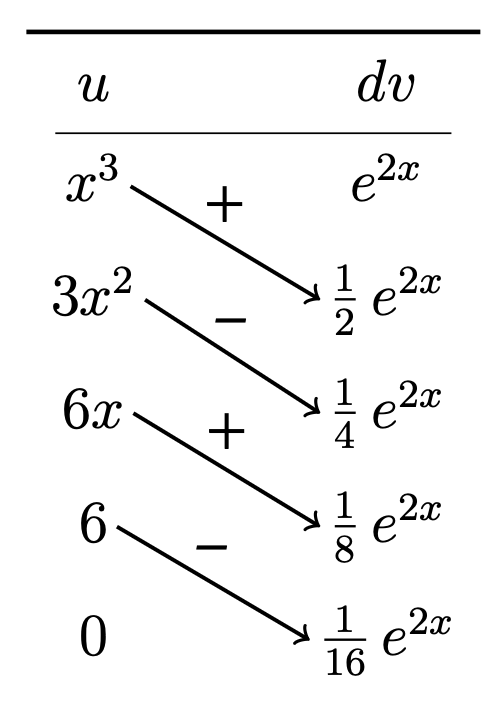
\includegraphics[width=0.19\textwidth]{images/tabular.png}
	\end{figure}
So that\dots
	\[
	\int x^3 e^{2x} \;dx= \dfrac{1}{2}\, x^3 e^{2x} - \dfrac{3}{4}\, x^2 e^{2x} + \dfrac{6}{8}\, x e^{2x} - \dfrac{6}{16} e^{2x} + C
	\]

\item Be able to compute integration-by-parts where one has to `loop back' to the original integral, i.e. `looping integrals'. 

\item Be able to recognize when an integral may be a `looping integral', e.g. $\ds\int e^x \sin x \;dx$ or $\ds\int \sin(2x) \cos x \;dx$, etc. This occurs most often when the integrand is of the form $\text{exponential} \cdot \text{trig}$ or $\text{trig} \cdot \text{trig}$ (but the trig functions have non-matching arguments).

\item Be able to use tabular integration to compute `looping' integrals, e.g. $\ds\int e^x \cos(2x) \;dx$
	\begin{figure}[H]
	\centering
	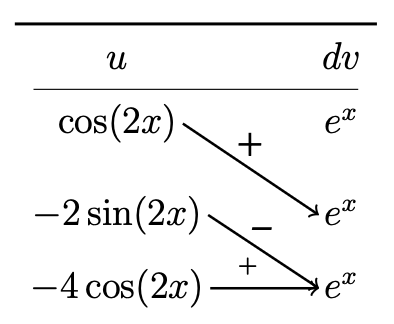
\includegraphics[width=0.22\textwidth]{images/looping.png}
	\end{figure}
So that\dots
	\[
	\begin{gathered}
	\int e^{x} \cos(2x) \;dx= e^x \cos(2x) + 2 e^x \sin(2x) - \int 4 e^x \cos(2x) \;dx \\[0.3cm]
	\int e^{x} \cos(2x) \;dx= e^x \cos(2x) + 2 e^x \sin(2x) - 4 \int e^x \cos(2x) \;dx \\[0.3cm]
	5 \int e^{x} \cos(2x) \;dx= e^x \cos(2x) + 2 e^x \sin(2x) + C \\[0.3cm]
	\int e^{x} \cos(2x) \;dx= \dfrac{1}{5} \left( e^x \cos(2x) + 2 e^x \sin(2x) \right) + C
	\end{gathered}
	\]

\item Be able to distinguish between integrals which require $u$-substitution, integration-by-parts, or both. 

\item Be able to compute some `shifting integrals' instead by integration-by-parts, e.g. $\ds\int x(2x + 1)^5 \;dx$ or $\ds\int \dfrac{x}{\sqrt{4x + 5}} \;dx$.
\end{itemize}

% 08/21, Thursday: Integration-by-Parts
\newpage
\section*{08/21, Thursday: Integration-by-Parts\label{08-21}}

\begin{itemize}
\item Know the integration-by-parts formula: $\ds\int u \;dv= uv - \int v \;du$, or in the case of a definite integral $\ds\int_a^b u \;dv= uv \bigg|_a^b - \int_a^b v \;du$.

\item Recall that the integration-by-parts formula comes from manipulating the product rule for derivatives, so it is a kind of `reverse product rule'.

\item Be able to use integration-by-parts to compute integrals. 

\item Recognize integrals where integration-by-parts may be appropriate, e.g. $\int x^2 \ln x \;dx$, $\ds\int x^2 e^{3x} \;dx$, $\ds\int \arctan x \;dx$, $\ds\int \ln x \;dx$, $\ds\int e^x \sin x \;dx$, etc. 

\item Be able to use LIATE and the `box method' to perform integration by parts, where\dots
	\begin{table}[H]
	\centering
	\begin{tabular}{rl}
	L: & Logarithms \\
	I: & Inverse Trig \\
	A: & Algebraic \\
	T: & Trigonometric \\
	E: & Exponential
	\end{tabular}
	\end{table}
One then creates a box and fills it in:
	\begin{figure}[H]
	\centering
	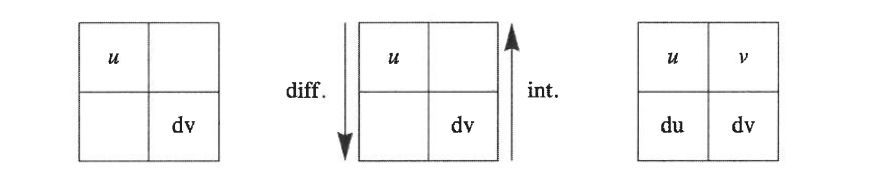
\includegraphics[width=0.80\textwidth]{images/box.png}
	\end{figure}
and then applies the `rule of 7':
	\begin{figure}[H]
	\centering
	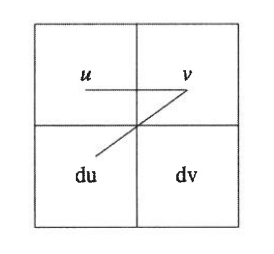
\includegraphics[width=0.20\textwidth]{images/7.png}
	\end{figure}
One can then write down $\ds uv - \int v \;du$. 

\item Know that the idea of integration-by-parts (by LIATE or otherwise) is to choose $dv$ to be the `hardest' part of the integrand that one can actually integrate, i.e. to simplify the integral by `integrating out' the hardest part possible and hope the resulting integral will be simpler. 

\item Know that LIATE can fail but often `overgrabs', i.e. $\ds\int x^3 e^{x^2} \;dx$ and how to fix it in this case. But also know that LIATE can fail completely, i.e. $\ds\int \dfrac{x e^x}{(1 + x)^2} \;dx$, and know how to `fix' $u$ and $dv$ in the case where LIATE totally fails. 

\item Be able to compute integrals where one first has to make a $u$-substitution before applying integration-by-parts, e.g. $\ds\int e^{\sqrt{x}} \;dx$ ($u= \sqrt{x}$), $\ds\int \sin(\sqrt[3]{x}) \;dx$ ($u= \sqrt[3]{x}$), etc.

\item Know that sometimes one has to perform integration-by-parts more than once to compute a given integral, e.g. $\ds\int x^2 e^x \;dx$ or $\ds\int x^3 \cos x \;dx$, or that some integration-by-parts integrals can `loop back' on themselves, e.g. $\ds\int e^x \sin x \;dx$ or $\ds\int \sin(2x) \cos(3x) \;dx$. 

\item Know that the integrals $\ds\int e^{x^2} \;dx$, $\ds\int \sin(x^2) \;dx$, and $\ds\int \cos(x^2) \;dx$ are all `impossible'. 
\end{itemize}

% 08/19, Tuesday: $u$-Substitution Review
\newpage
\section*{08/19, Tuesday: $u$-Substitution Review\label{08-19}}

\begin{itemize}
\item Know that $\ds\int_a^b f(x) \;dx$ represents the net area `under the curve' $f(x)$ between $x= a$ and $x= b$, i.e. the net directed area between $f(x)$ and the $x$-axis between $x= a$ and $x= b$---area under the $x$-axis counting as negative.

\item Know that if $\ds\int f(x) \;dx= F(x)$, then $\ds\int_a^b f(x) \;dx$ computes the net change in $F(x)$ between $x= a$ and $x= b$, i.e. $\ds F(b) - F(a)= \int_a^b f(x) \;dx$.

\item Memorize the `elementary' integrals:
	\begin{2itemize}
	\item $\ds\int \# \;dx= \#x + C$
	\item $\ds\int x^n \;dx= \dfrac{x^{n+1}}{n+1} + C, n \neq -1$
	\item $\ds\int \dfrac{1}{x} \;dx= \ln|x| + C$
	\item $\ds\int \sin x \;dx= -\cos x + C$
	\item $\ds\int \cos x \;dx= \sin x + C$
	\item $\ds\int \tan x \;dx= \ln|\sec x| + C$
	\item $\ds\int \sec x \;dx= \ln|\sec x + \tan x| + C$
	\item $\ds\int \csc x \;dx= \ln|\csc x - \cot x| + C$
	\item $\ds\int \cot x \;dx= \ln|\sin x| + C$
	\item $\ds\int \sec^2 x \;dx= \tan x + C$
	\item $\ds\int \sec x \tan x \;dx= \sec x + C$
	\item $\ds\int \csc^2 x \;dx= -\cot x + C$
	\item $\ds\int e^x \;dx= e^x + C$
	\item $\ds\int a^x \;dx= \dfrac{a^x}{\ln a} + C$
	\item $\ds\int \ln x \;dx= x \ln x - x + C$
	\item $\ds\int \log_b x \;dx= \dfrac{x \log_b x - x}{\ln b} + C$
	\item $\ds\int \dfrac{1}{1 + x^2} \;dx= \arctan x + C$
	\item $\ds\int \dfrac{1}{\sqrt{1 - x^2}} \;dx= \arcsin x + C$
	\end{2itemize}

\item Know when $u$-substitution might be appropriate: when one has a function one can integrate but is `off' by a factor whose derivative (up to a multiple) is in the integrand. For example, $\ds\int x e^{x^2} \;dx$. Here we know how to integrate $e^x$ but is `off' by $x^2$, whose derivative $2x$ can be found (up to a multiple) in the integrand, i.e. the $x$.

\item Know how to use $u$-substitution with both definite and indefinite integrals, e.g. $\ds\int \dfrac{\sin(\ln x)}{x} \;dx$ and $\ds\int_1^4 \dfrac{e^{\sqrt{x}}}{\sqrt{x}} \;dx$.

\item Be able to perform linear $u$-substitution in your head, i.e. one should be able to compute integrals `like' $\ds\int e^{3x} \;dx$, $\ds\int \sin\left( \tfrac{x}{2} \right) \;dx$, $\ds\int (2x - 1)^5 \;dx$, etc. in one's head. 

\item Remember to always change your bounds when performing $u$-substitution with a definite integral!

\item Recognize the special case of $u$-substitution of `shifting' integrals, where one needs to solve for $x$ in $u= \cdots$, e.g. $\ds\int \dfrac{x}{x + 3} \;dx$, $\ds\int x \sqrt{x - 2} \;dx$, $\ds\int 4x(x + 3)^{10} \;dx$, etc. 
\end{itemize}

\end{document}